\section{Durchführung}
\subsection{Aufbau}
\label{sec:Durchführung}
Der Aufbau besteht hauptsächlich aus einer optischen Strecke. Das Licht einer Spektrallampe wird gebündelt und auf $\lambda = \SI{794,8}{\nano \meter}$
gefiltert. Das entspricht der $\mathrm{D}_1$ Linie von Rubidium, welches untersucht wird. Mit einer Kombination aus einem Polarisationsfilter und einer
$\sfrac{\lambda}{4}$-Platte wird das Licht rechtszirkular polarisiert. Dieses Licht durchquert eine Dampfzelle, in der eine Mischung aus ${}^87\mathrm{Rb}$
und ${}^87\mathrm{Rb}$ gasförmig vorliegt. Die Dampfzelle ist beheizt, um einen optimalen Dampfdruck zu erzeugen. Das austretende Licht wird erneut gebündelt
und von einem Photoelement gemessen. Die optischen Bauteile werden so justiert, dass die Intensität am Photoelement maximal ist. Die Dampfzelle ist von drei Helmholtzspulen umgeben, von denen zwei zum ausgleich des Erdmagnetfeldes sind und eine für
die eigentliche Messung. Dieser Aufbau ist in Abbildung \ref{fig:aufbaucom} skizziert.
\begin{figure}
	\centering
	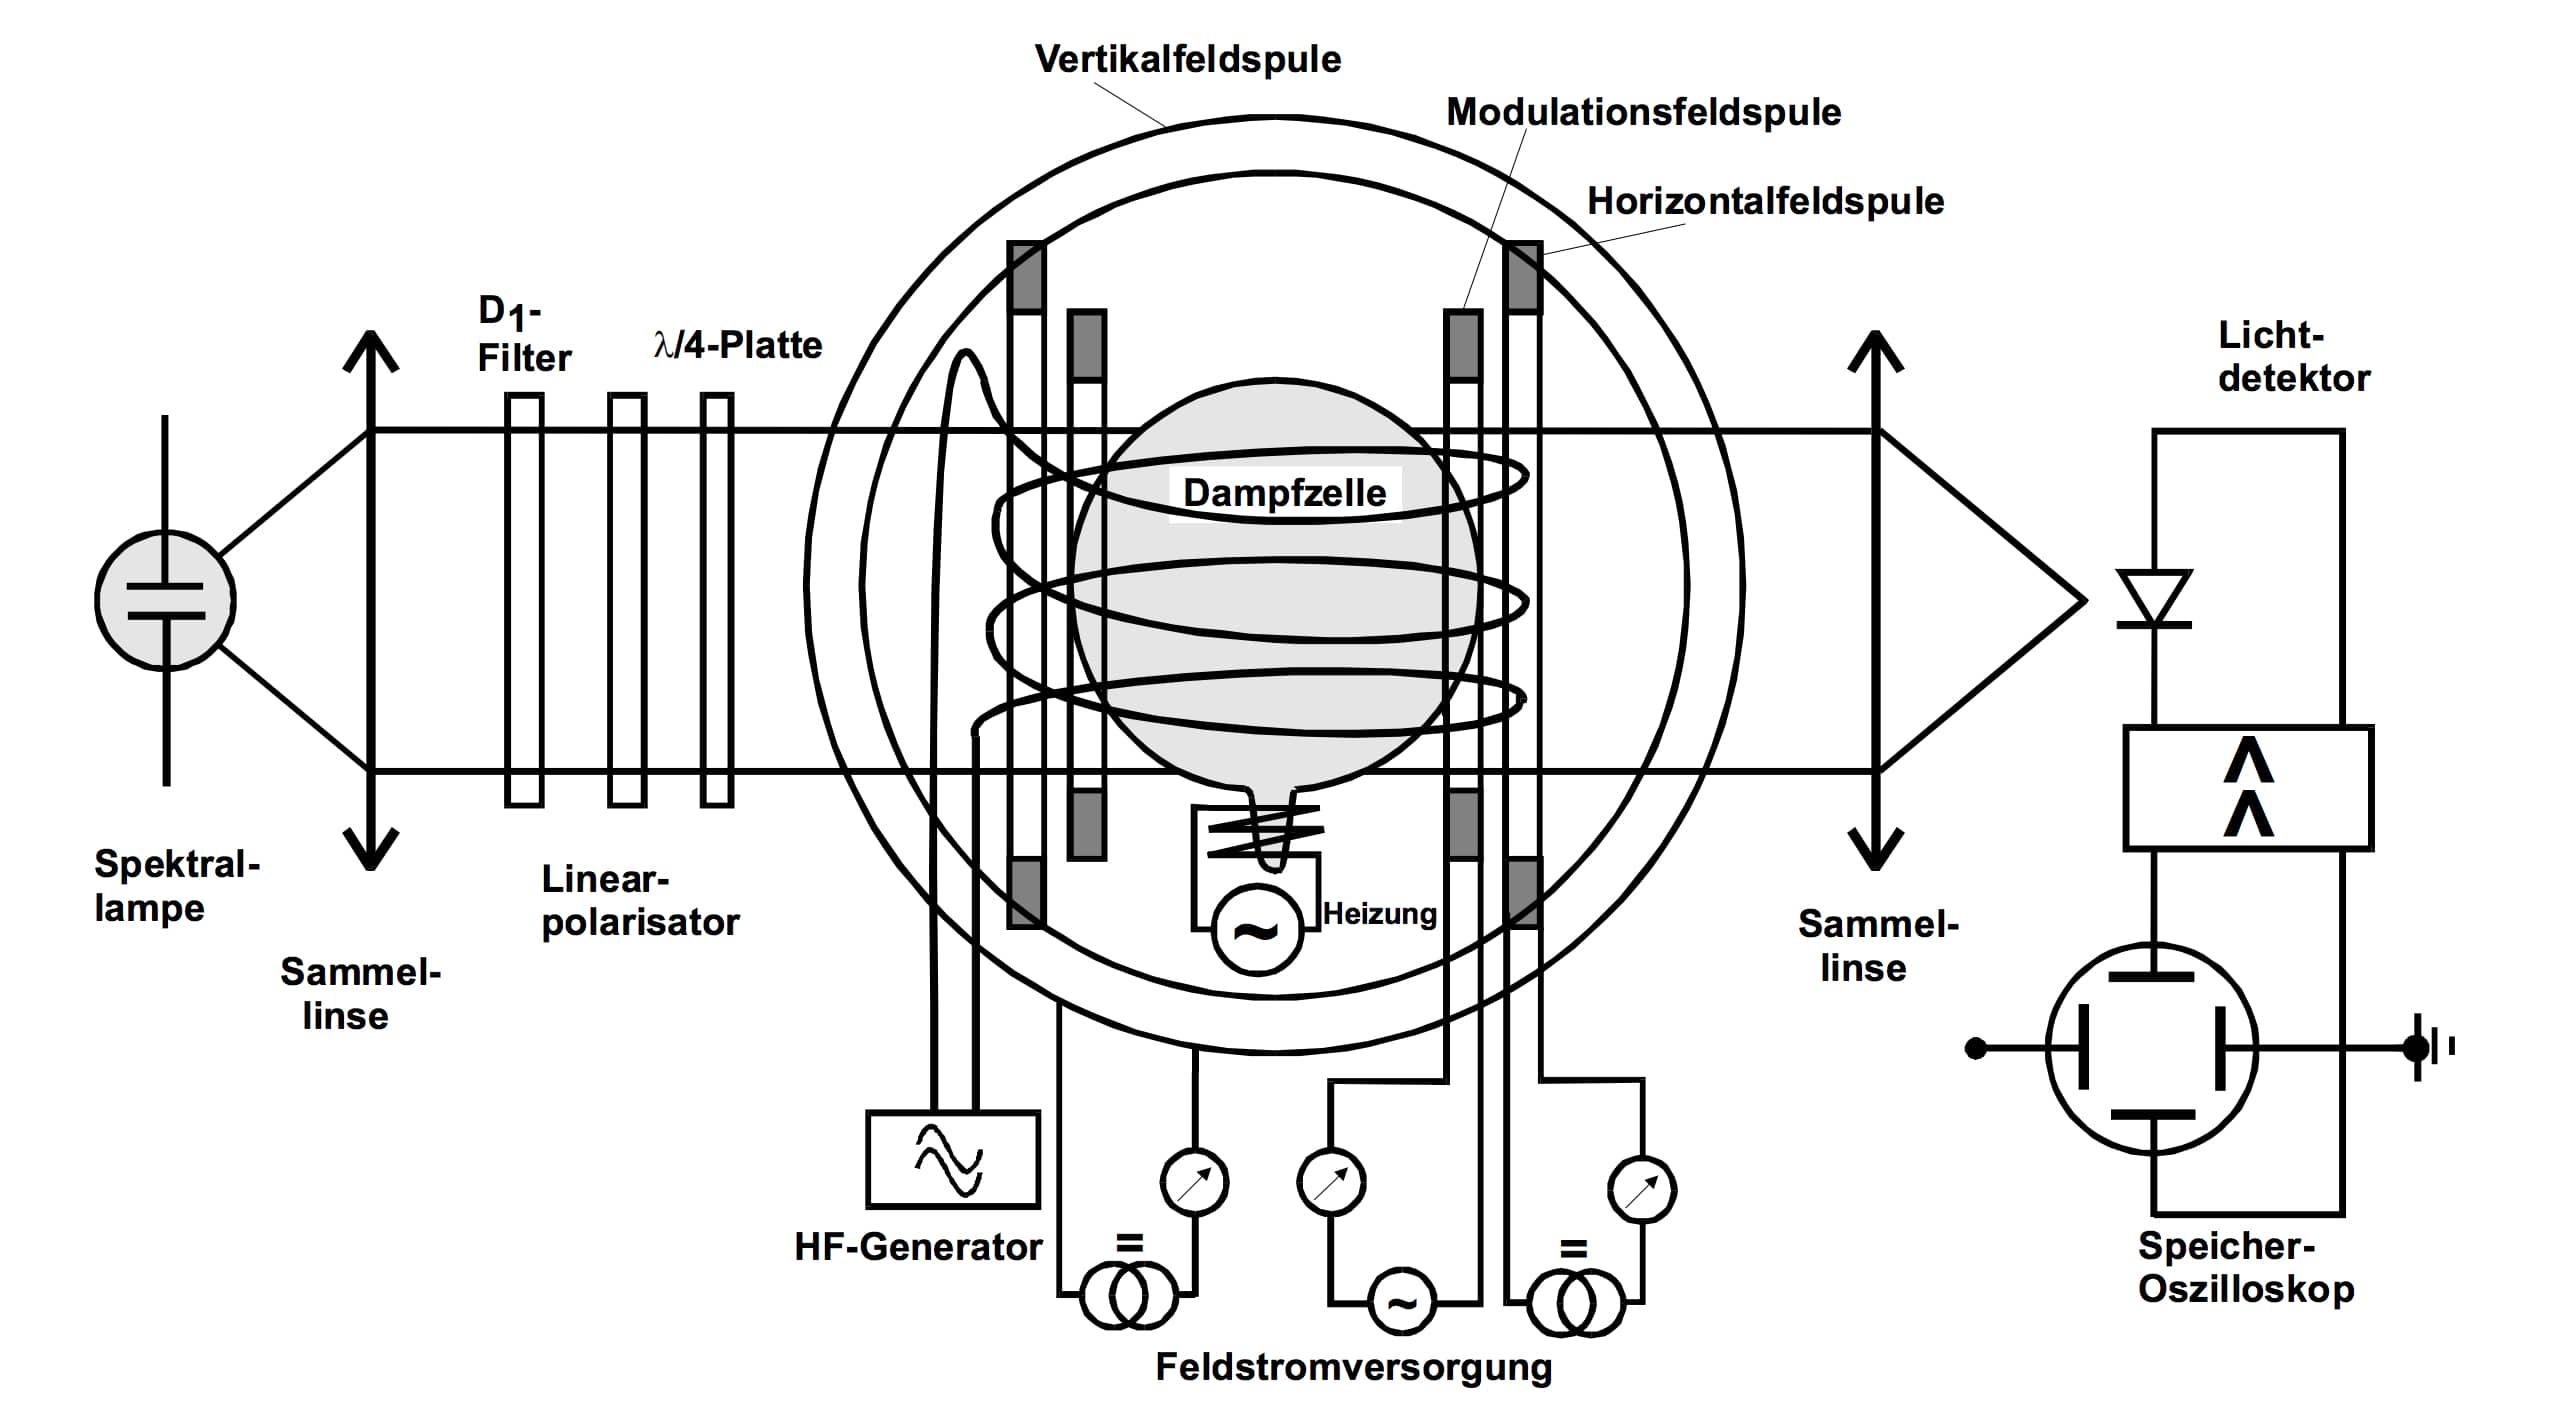
\includegraphics[width=0.8\linewidth]{img/aufbaucom.jpg}
	\caption{Schematischer Aufbau des optischen Pumpens.\cite{V21}}
	\label{fig:aufbaucom}
\end{figure}
Der Aufbau wird so gedreht, dass die Lichtstrecke in Nord-Süd Richtung verläuft. Dadurch wird der Einfluss des Horizontalen Erdmagnetfeld minimiert.
Nun wird die RF-Spule eingeschaltet und bei konstanter Frequenz gehalten. Zusätzlich wird bei einer horizontales Spule die Magnetfeldstärke variert. Bei der
Resonanzfeldstärke fällt die Transperenz der Dampfzelle stark, da jetzt die Photonen die richtige Energie zum optischen Pumpen haben. Wenn man die Transperenz
gegen die Feldstärke aufträgt, ist ein breiter Dip zu sehen. Dieser wird schmaler, umso besser das Erdmagnetfeld ausgeglichen wird. Dazu gibt es eine
Vertiklale Spule und die Orientierung des Aufbaus.
\subsection{Messablauf}
Es wird die horizontale Magnetfeldstärke gegen die Frequenz der RF-Spule aufgenommen. Die Frequenz soll zwischen $\SI{100}{\kilo \hertz}$ und $\SI{1}{\mega \hertz}$ variert werden. Für höhere Frequenzen ($>\SI{200}{\kilo \hertz}$) kann es nötig sein, ein konstantes Magnetfeld zusätlich als "offset dazu zunehmen.
Um das Verhältnis der Rb-Isotobe zu bestimmen, wird ein Bild dess Osziloskop aufgenommen, auf dem die zwei Dips der Transperenz zu sehen sind.
